\chapter{Algebra}

\section{Q1}

  A mixture of 12 ounces of vinegar and oil is 40 percent vinegar, where all
  of the measurements are by weight. How many ounces of oil must be added to
  the mixture to produce a new mixture that is only 25 percent vinegar?

  \subsection{解析}

    \begin{align*}
      v &= 12 \times 0.4 \\
      &= 4.8 \\
      \frac{4.8}{12 + x} &= 0.25 \\
      x &= 0.72
    \end{align*}

    mixture的重量是所有组成部分的总和

\section{Q2}

  What is the y-intercept of the graph of the equation
  $ y = 2 \times \left| 4x − 4 \right| − 10 $

  \subsection{解析}

    \textbf{已知x, 求y, 只有一种情况 (如果是已知y, 求x, 则有两种情况)}

    \begin{align*}
      y &= 2 \times \left| 4x − 4 \right| − 10 \\
      &= 2 \times \left( -4 \right) - 10 \\
      &= -2
    \end{align*}

\section{Q3}

  Line l passes through points in both quadrants II and III.
  Which of the following statements are true?
  \textbf{Indicate all such statements.}

  \begin{enumerate}
    \item Line l cannot pass through the origin.
    \item Line l cannot pass through any point in quadrant I.
    \item Line l cannot pass through any point in quadrant IV.
    \item The slope of line l cannot be 0.
    \item The slope of line l cannot be positive.
    \item The slope of line l cannot be negative.
  \end{enumerate}

  \subsection{解析}

    \textbf{本题只提到了过 Quadrant 2, 3, 没有提到 l 没过 1, 4}

    \begin{enumerate}
      \item \textbf{正确}: 过原点
      \item \textbf{错误}: 没提
      \item \textbf{错误}: 没提
      \item \textbf{正确}: 斜率为0没发过x轴
      \item \textbf{错误}: 同 2.
      \item \textbf{错误}: 同 3.
    \end{enumerate}

\section{Q4}

  Line L in the xy-plane contains points A and B with coordinates
  $ (-4, 5) $ and $ (6, -1) $, respectively.
  Line k is perpendicular to L and contains the midpoint of line segment AB.
  Which of the following statements are true? Indicate all such statements.

  \begin{enumerate}
    \item The slope of line l is $ -3/5 $.
    \item Line k has a negative slope.
    \item Line k contains the point $ (1,2) $.
  \end{enumerate}

  \subsection{解析}

    \begin{enumerate}
      \item \textbf{正确}: 根据A, B可知
      \item \textbf{错误}: 1. 的负倒数是正数
      \item \textbf{正确}: L的中点是 $ (1, 2) $
    \end{enumerate}

\section{Q5}

  What is the sum of all possible solutions to the equation

  \begin{align*}
    \sqrt{2x^{2} - x - 9} &= x + 1 \\
    x^{2} - 3x - 10 &= 0 \\
    x &= -2, 5
  \end{align*}

  \subsection{解析}

    \textbf{x不能等于$ -2 $, 不然等号左面不行, 所以 $ x = 5 $, $ \sum = 5 $}

\section{Q6}

  \begin{figure}[H]
    \centering
    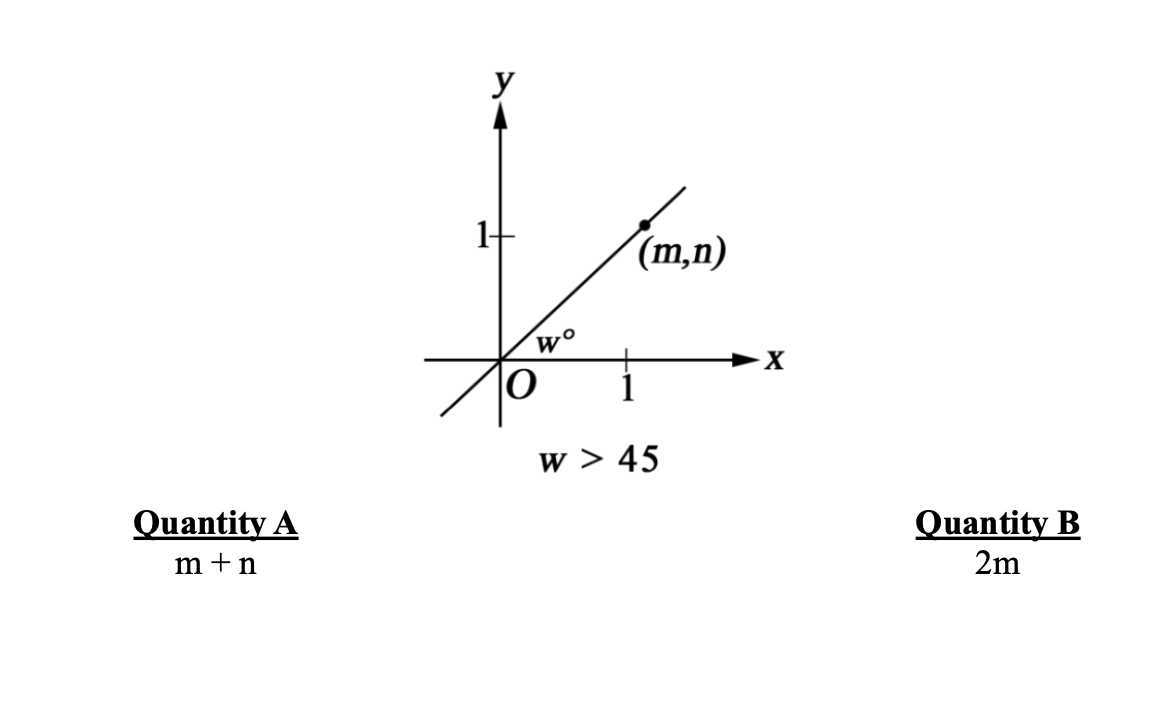
\includegraphics[width=0.7\columnwidth]{images/areas/algebra/q6}
  \end{figure}

  \subsection{解析}

    \textbf{本题注意解析图示, $ \left( m, b \right) $在第一象限, 且$ m > 1, n > 1 $}
    $ n > m $, 所以$ m + n > 2m $

\section{Q7}

  The quadratic function $ f\left( x \right) = -k^{2}x^{2} - mkx - \frac{1}{16} $
  where $ m, k $ are constants, does not have any intersection with x-axis.
  In which of the following interval of $ m $ the statement given above
  does not necessarily hold true?

  \begin{enumerate}
    \item $ - \frac{9}{16} < m < - \frac{7}{16} $
    \item $ - \frac{7}{16} < m < - \frac{5}{16} $
    \item $ \frac{1}{16} < m < \frac{1}{16} $
    \item $ \frac{1}{16} < m < \frac{3}{16} $
    \item $ \frac{3}{16} < m < \frac{5}{16} $
  \end{enumerate}

\section{Q8}

  \begin{equation*}
    \left( x + 3 \right) \left( y - 4 \right) = 0
  \end{equation*}

  \begin{itemize}
    \item \textbf{Quantity A}: $ x y $
    \item \textbf{Quantity B}: $ - 12 $
  \end{itemize}

  \subsection{解析}

    \textbf{本题注意有连个变量, 只要$ x = -3 $或者$ y = 4 $任意一个达成就行, 所以
    无法分析, D}

